% For formatting purposes only 
\setcounter{chapter}{5}
\setcounter{section}{7}
%\listofalgorithms - think about it ...
%--------------
%- COPY START -
%--------------        
\subsection{(W/R) Rule Implementation}\label{sec:ruleImplementation}
\begin{itemize}
    \item Make references to \emph{decision points} in avoidance algorithm and navigation loop
    \item define context state based on \emph{decision points}.
    \item Short roadmap to rules,
\end{itemize}
\begin{figure}[H]
    \centering
    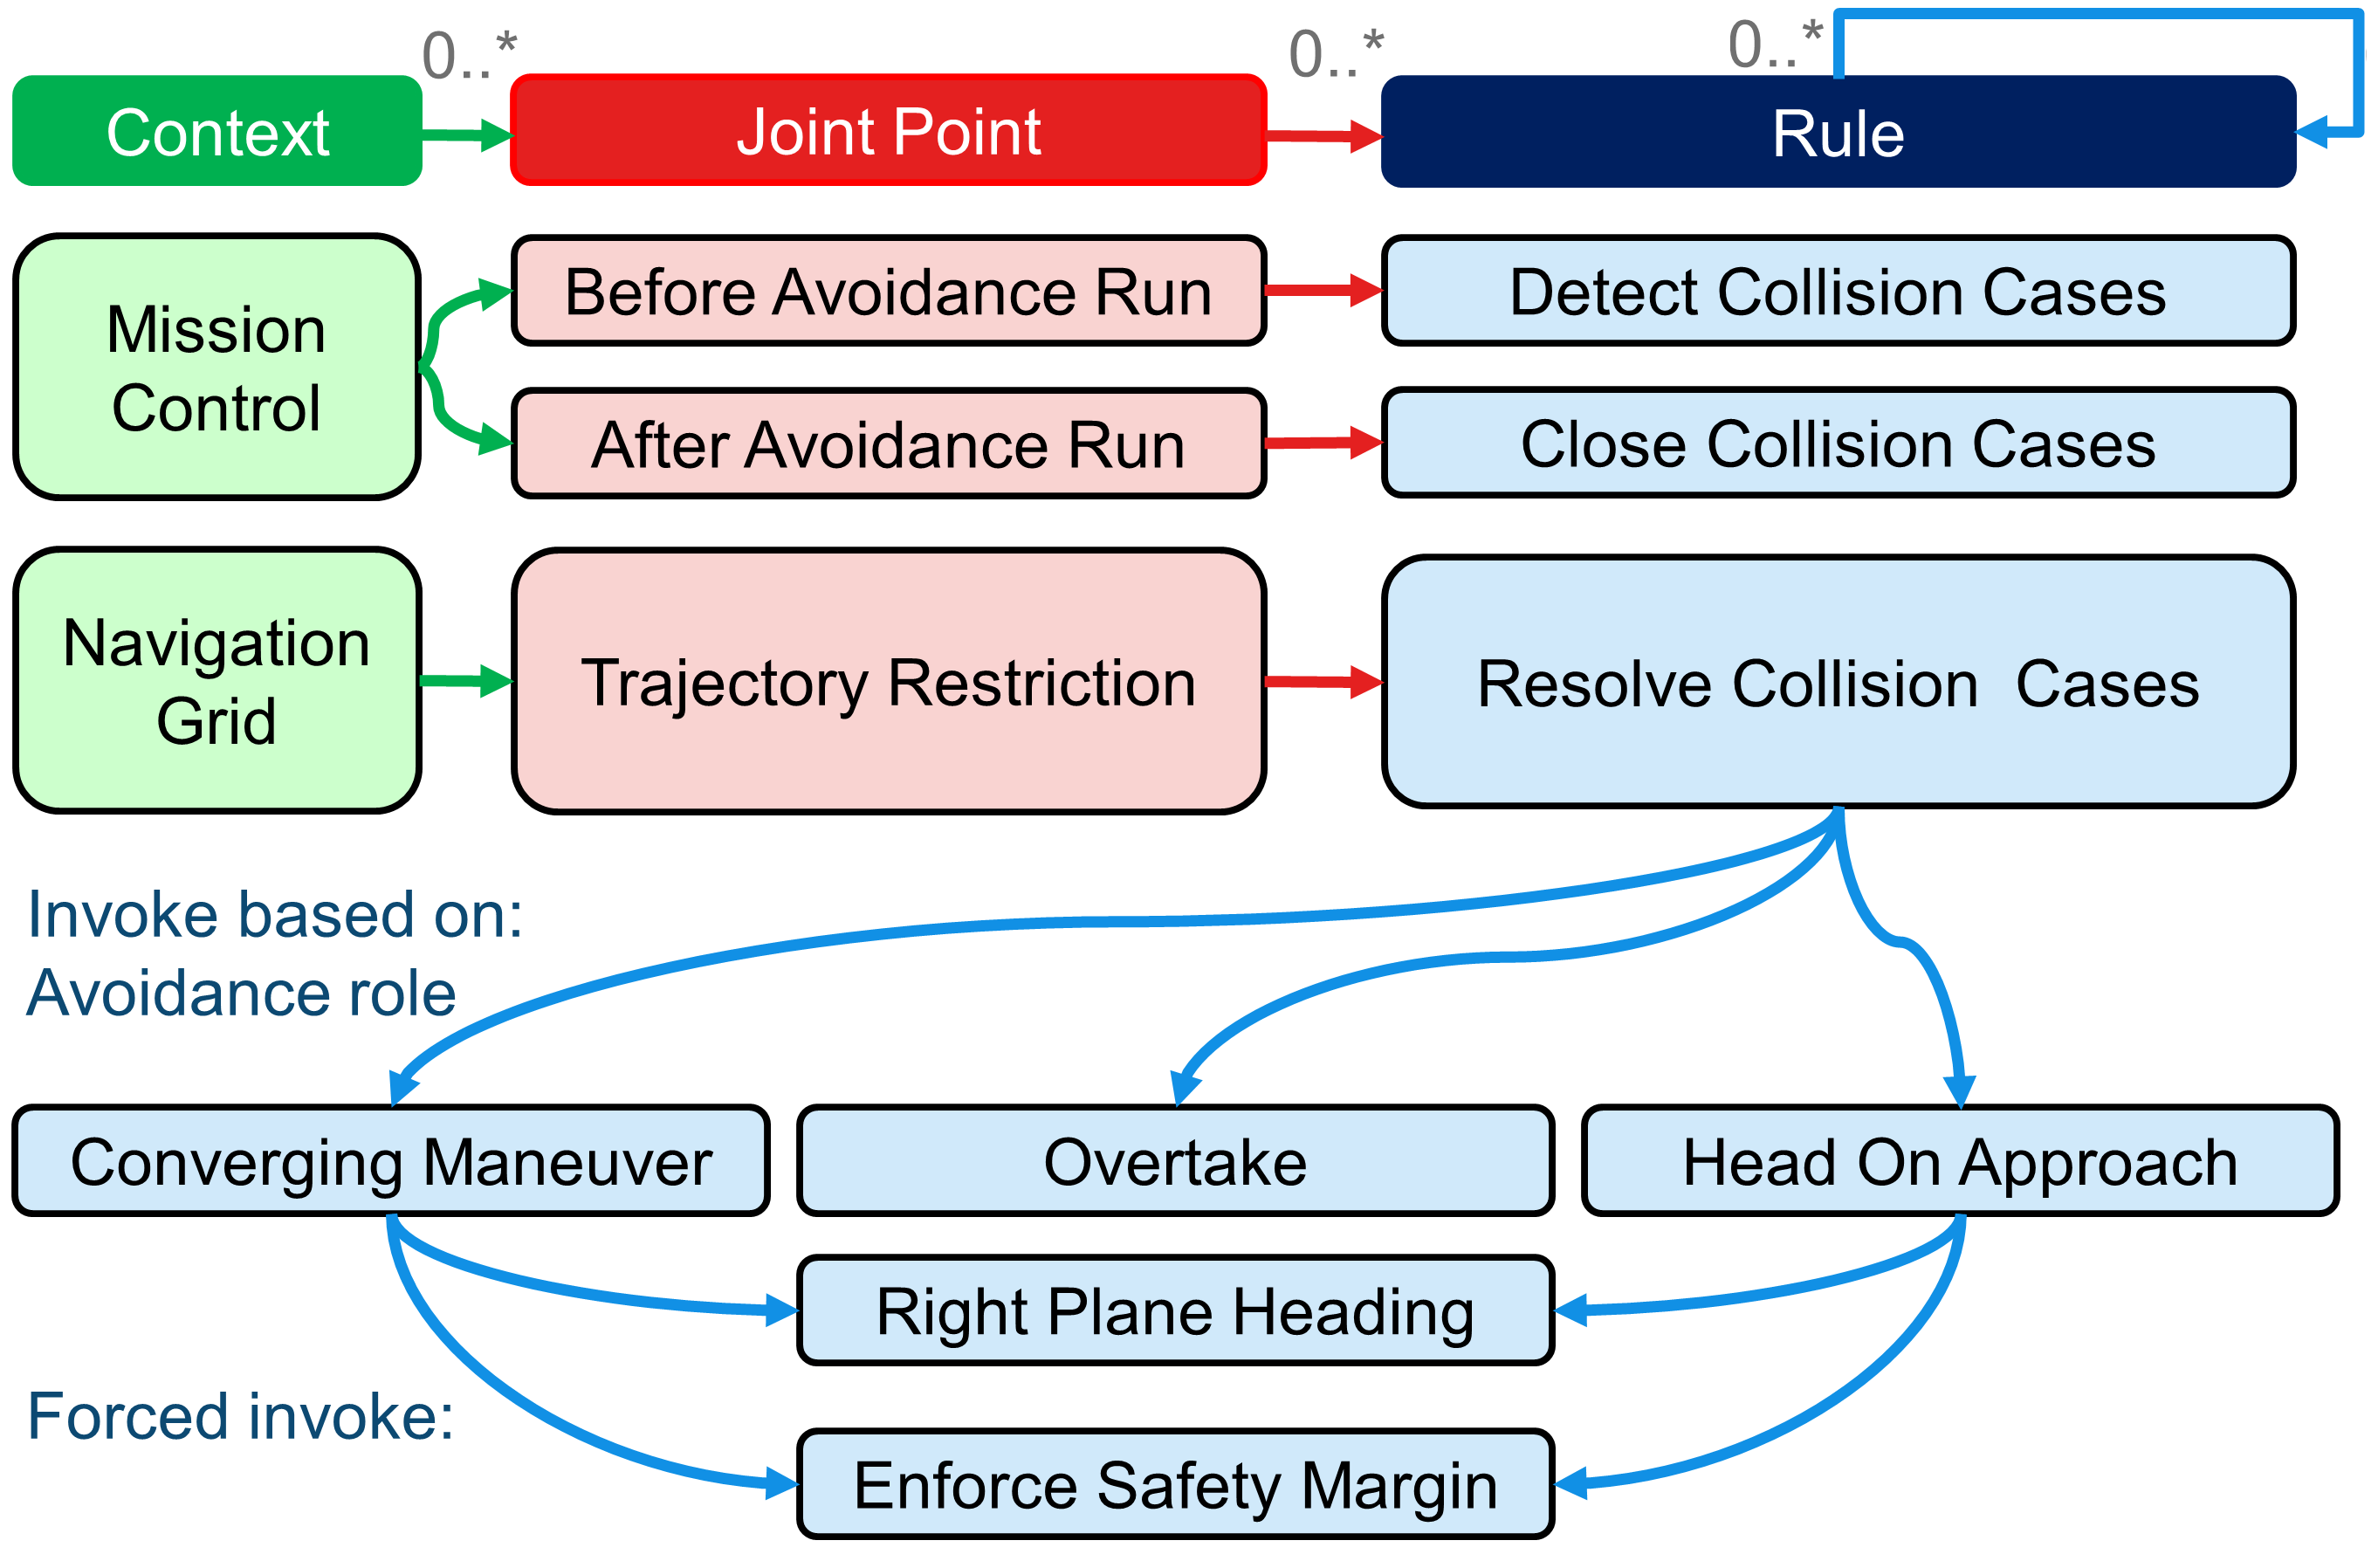
\includegraphics[width=0.7\linewidth]{\FIGDIR/RE014RuleEngineInstanceLevels} 
    \caption{Rule engine initialization with Rules of the air.}
    \label{fig:RuleEngineInstanceLevels}
\end{figure}

\subsection{Rule: Detect Collision Cases}
    \noindent This rule is activated each \emph{UAS avoidance run}. \emph{UTM} sent out all related \emph{collision cases} (\ref{eq:fetchCollisionCases}) based on our \emph{UAS identifier}. Creation of \emph{collision case} is given in sec. \ref{sec:collisionCase} based on air traffic periodical\emph{position notifications} (sec \ref{sec:positionNotification}).
    \begin{equation}\label{eq:fetchCollisionCases}
        UTM\times timeFrame \to UTMCollisionCases
    \end{equation}
    
    If there are available \emph{position notifications} (sec \ref{sec:positionNotification}) from surrounding air-traffic, UAS will calculate own \emph{collision cases} (\ref{eq:createUASCollisionCases}).
    \begin{equation}\label{eq:createUASCollisionCases}
        uasStatus\times positionNotification\times utmTimeFrame\to UASCollisionCases
    \end{equation}
    
    Then UAS merges \emph{own collision cases} with \emph{UTM collision cases}, if there exist following disparities UAS will take action:
    \begin{enumerate}
        \item $distamce(ownCollisionPoint,utmCollisionPoint)\ge threshold$, send UTM notificaiton, use \emph{utmCollisionPoint}
        \item $utmMargin \ge ownMargin$, use safety margin from UTM.
        \item $utmAvoidanceRole == active, ownAvoidanceRole == inactive$, use UTM avoidance role.
        \item $utmCollisionCase == active, ownCollisionCase == uncertain$, use UTM provided collision case, not all \emph{position notifications} are available. 
        \item $utmCollisionCase == inactive, ownCollisionCase == active$, notify UTM with new collision case, ignore collision case until UTM approves.
    \end{enumerate}
    \begin{note}
        \emph{Avoidance role} is classified as \emph{inactive} if and only if UAS has \emph{right of the way}, it is classified as \emph{active} otherwise.
        
        \emph{Safety margin} determined by UTM has priority, because not all calculations factors are available for UAS.
        
        \emph{Collision Case} unknown to UTM are ignored, due to safety reasons (false data spoofing), collison case is activated after UTM confirmation. If there is real intruder not confirmed by UTM it is handled via \emph{non-cooperative} or \emph{emergency} avoidance procedure
    \end{note}
    
    \emph{Selection process} of active \emph{collision cases} is based on UAS \emph{avoidance role} in each \emph{collision case}.
    \begin{itemize}
        \item If the \emph{avoidance roles} are following: \emph{Head On Approach, Converging Maneuver, or Overtake} in all \emph{collision cases} UAS system will stay in cooperative mode.
        \item If there exists at least one \emph{collision case} with \emph{own avoidance role} or \emph{intruder avoidance role} set as \emph{emergencing}, the UAS will notify UTM and ask for \emph{diversion order}, meanwhile it sets itself into \emph{Emergency avoidance} mode.
        \item If there exist multiple \emph{Overtake avoidance roles} or combination of \emph{Overtake avoidance role} and \emph{Other active role}, the UAS will decrease its cruising speed like follows:
        \begin{equation}
            UASSpeed = \max \left\{\begin{aligned}
            & minimalUASCruisingSpeed,\\
            &\min \left\{intruderSpeed\right\}\quad \forall activeCollisionCases
            \end{aligned}
            \right\}
        \end{equation}
        During \emph{slow-down} UAS switchs to \emph{emergency avoidance mode} and asks for \emph{divergence order} from UTM.
    \end{itemize}
    
    \emph{Ordering of collision cases} starts if and only if the \emph{UAS} is in \emph{cooperative avoidance mode}. The cases are ordered for processing based on severity rating which is calculated based on:
    \begin{enumerate}
        \item \emph{Safety Margin} - the greater safety margins are prioritized.
        \item \emph{Intruder vehicle class} - the more dangerous intruders are prioritized.
        \item \emph{Collision point distance} - closer collision points are prioritized.
        \item \emph{UAS avoidance role} - \emph{Head on Approach} is favored upon \emph{Converging maneuver}, due to direct collision severity.
    \end{enumerate}
    
    \emph{Rule engine invocation} for each \emph{active collision case} is then applied on \emph{descending severity sorted} list. 
    
    The rule is summarized in table \ref{tab:ruleDetectCollisionCases}.
    
    \begin{tabularx}{\textwidth}{|X|X|X|}
    \hline\multicolumn{3}{|X|}{
        \begin{minipage} [t] {0.95\textwidth} 
            \emph{Invocation:} Every \emph{Decision point} in\emph{UAS main loop}\\\\
            \emph{Objective:}
            \begin{enumerate}
                \item Fetch UTM \emph{Collision cases} for given decision time frame.
                \item Create/update own \emph{own collision cases} based on received \emph {Position notifications} from surrounding \emph{Intruders}.
                \item Merge \emph{Collision cases} based on \emph{UTM priority order}.
                \item Select active \emph{collision cases} based on following conditions:
                \begin{enumerate}[a.]
                    \item \emph{Active participation} in \emph{collision case} where \emph{avoidance role} $\neq$ \emph{Right of the way}.
                    \item \emph{Collision point} is int front of UAS.
                    \item \emph{Emergency mode detection} there exist at least one non-cooperative participant.
                \end{enumerate}
                \item Order \emph{collision cases} based on \emph{severity}.
                \item If there is at least one \emph{active collision case} enforce rule \emph{Resolve collision case} (tab \ref{tab:ruleResolveCollisionCase})  for each \emph{active collision case}.
            \end{enumerate}
            \rule{0pt}{0pt}
        \end{minipage}}\\
    \hline%\multicolumn{3}{X|}{Context & Condition & Application}\\
    \hline
        \emph{Context} & \emph{Condition} & \emph{Application}\\
    \hline
        \begin{minipage} [t] {0.3\textwidth}
            UAS Mission control,\\
            Before Avoidance Run,\\
            UTM/UAS collision cases\\
            \vspace{2mm}
        \end{minipage}&
        \begin{minipage} [t] {0.3\textwidth}
            Clean \emph{avoidance grid},\\
            No emergency
            \vspace{2mm}
        \end{minipage}&
        \begin{minipage} [t] {0.3\textwidth}
            Active collision case selection, Prioritization
            \vspace{2mm}
        \end{minipage}\\
    \hline
            \caption{Detect collision cases rule definition.}
    \label{tab:ruleDetectCollisionCases}
    \end{tabularx}

\subsection{Rule: Resolve Collision Case}\label{sec:ruleResolveCollisionCase}
    \noindent\emph{Active collision cases} are processed one by one. All collision cases are applied to \emph{Navigation grid}. \emph{Navigation grid} contains all possible \emph{trajectories} in form of \emph{Reach set}. All \emph{trajectories} are \emph{reachable} at the beginning of UAS \emph{avoidance frame}. Each application of \emph{collision case resolution} rule disables some subset of feasible \emph{trajectories}. For this reason are \emph{active collision cases} sorted by severity. 
    
    It is assumed that UAS is in \emph{cooperative avoidance mode}. If previous application of this rule forced UAS into \emph{emergency mode} the rule is not applied to save system resources. \emph{Emergency} mode is invoked if \emph{rule application} disable all \emph{trajectories} in \emph{Navigation grid}. If there is at least one \emph{feasible trajectory} in \emph{avoidance grid} follow-up rule is invoked based on UAS \emph{avoidance role}.
    
    The rule is summarized in table \ref{tab:ruleResolveCollisionCase}.
    
    \begin{tabularx}{\textwidth}{|X|X|X|}
    \hline\multicolumn{3}{|X|}{
        \begin{minipage} [t] {0.95\textwidth} 
            \emph{Invocation:} This rule is invoked if exists at least one \emph{active collision case} in given \emph{navigation grid time-frame}, moreover \emph{avoidance grid} must be empty and \emph{cooperative avoidance mode} is enforced.\\\\
            \emph{Objective:} Based on \emph{active collision case} and \emph{UTM directives} enforce behaviour based on \emph{own avoidance role}:
            \begin{enumerate}
                \item \emph{Head on approach} - rule \ref{tab:ruleHeadonApproach}.
                \item \emph{Converging maneuver} - rule \ref{tab:ruleConvergingManuever}.
                \item \emph{Overtake} - rule \ref{tab:ruleOvertakeDefinition}.
                \item \emph{Emergency mode} - switch from \emph{active avoidance mode} to \emph{emergency mode}.
            \end{enumerate}
            \rule{0pt}{0pt}
        \end{minipage}}\\
    \hline%\multicolumn{3}{X|}{Context & Condition & Application}\\
    \hline
        \emph{Context} & \emph{Condition} & \emph{Application}\\
    \hline
        \begin{minipage} [t] {0.3\textwidth}
            UAS mission control,
            Trajectory restriction,
            Collision cases,
            \vspace{2mm}
        \end{minipage}&
        \begin{minipage} [t] {0.3\textwidth}
            Active merged collision case, Resolution mandate from UTM
            \vspace{2mm}
        \end{minipage}&
        \begin{minipage} [t] {0.3\textwidth}
            \centering
            Enforce Rules of Air\\
            or\\
            Enforce emergency
            \vspace{2mm}
        \end{minipage}\\
    \hline
            \caption{Resolve collision case rule definition.}
    \label{tab:ruleResolveCollisionCase}
    \end{tabularx}

\subsection{Rule: Close Collision Cases}\label{sec:ruleCloseCollisionCases}    
    \noindent\emph{Collection of rule results} detected by rule \ref{tab:ruleDetectCollisionCases} and \emph{resolved} by rule \ref{tab:ruleResolveCollisionCase} is done via \emph{context of rule engine}. For each \emph{time-frame} and each $trajectory\in NavigationGrid$, there exists rule engine \emph{context} query (\ref{eq:collectFromContextClosingCollisionCases}) which returns \emph{trajectory status} and \emph{list of applied rules on trajectory}.
    \begin{equation}\label{eq:collectFromContextClosingCollisionCases}
        Context(trajectory,timeFrame) \to \left\{State: Enabled/Disabled, Rule(s)\right\}
    \end{equation}
    
    \emph{Calculation of possible trajectories} in \emph{navigation grid} is using \emph{collected rule results} (\ref{eq:collectFromContextClosingCollisionCases}). If the \emph{trajectory state} and linked \emph{rule reason} is sufficient, the \emph{trajectory} is disabled for given \emph{time frame}. \emph{Standard navigation algorithm} (TBD - reference to section with outer navigaiton loop) is used to select \emph{feasible trajectory}. 
    
    \emph{Rules of the air} and their applicaiton in \emph{General Aviation} cases is consistent. Increasing trafic density can impose new layers of rules, which may cause the \emph{soft deadlock} in \emph{manuverability}. In this case \emph{Navigation grid} will have all  \emph{possible trajectories} exhausted. Following procedure is executed:
    \begin{enumerate}
        \item UAS switch into \emph{Non-cooperative avoidance mode} or \emph{Emergency avoidance mode} depending on situation severity (One conflict can be handled with \emph{vertical separation} of conflicting aircrafts).
        \item UAS broadcasts \emph{warning message} to all nearby aircrafts, and \emph{separation message(s)} to conflicting aircraft. \emph{Separation message} contains \emph{expected collision point} and \emph{preferred separation type}.Each conflicting aircraft then reacts and sends \emph{action notification} to UTM.
        \item If UAS switchs into \emph{emergency mode}, non cooperative avoidance using \emph{avoidance grid} is induced. Each relevant intruder is projected as \emph{timed body volume intruder} (TBD reference to intruder probabilistic model), where \emph{safety margin} is used as \emph{body radius}.
    \end{enumerate}
    
    \emph{UAS} notifies \emph{UTM} with \emph{course change}, \emph{planned avoidance trajectory}, \emph{avoidance mode}. \emph{UTM} approves planned changes or sends \emph{plan corrections} (out of scope). The rule summary is given in table \ref{tab:ruleCloseCollisionCase}
    
    
    \begin{tabularx}{\textwidth}{|X|X|X|}
    \hline\multicolumn{3}{|X|}{
        \begin{minipage} [t] {0.95\textwidth} 
            \emph{Invocation:} There exists at least one \emph{active collision case} which had impact on \emph{Navigation grid}.\\\\
            \emph{Objective:} Ensure that multiple \emph{avoidance rules} application gives feasible \emph{avoidance strategy}, enter into \emph{emergency avoidance mode} otherwise. Following steps are executed:
            \begin{enumerate}
                \item \emph{Collect rules} applied on \emph{navigation grid} from \emph{active collision cases}.
                \item \emph{Calculate possible trajectories for avoidance}, there may be none.
                \item If there is no \emph{feasible route}, for each \emph{intruder} from related \emph{collision cases}:
                \begin{enumerate}[a.]
                    \item Issue \emph{warning message} containing \emph{expected collision point} and \emph{preferred separation type}.
                    \item Create appropriate \emph{intruder object} for \emph{avoidance grid}.
                    \item Calculate \emph{evasive maneuver} based on expected \emph{separation type}.
                \end{enumerate}
                \item \emph{Notify UTM} with \emph{collision case resolution} for each \emph{active collision case}.
                \emph{Nofigy UTM} with \emph{planned trajectory} and \emph{avoidance mode}
            \end{enumerate}
            \rule{0pt}{0pt}
        \end{minipage}}\\
    \hline%\multicolumn{3}{X|}{Context & Condition & Application}\\
    \hline
        \emph{Context} & \emph{Condition} & \emph{Application}\\
    \hline
        \begin{minipage} [t] {0.3\textwidth}
            UAS Mission control,\\
            After avoidance run,\\
            Collision resolutions
            \vspace{2mm}
        \end{minipage}&
        \begin{minipage} [t] {0.3\textwidth}
            At least one trajectory in Navigation grid,\\
            Emergency check
            \vspace{2mm}
        \end{minipage}&
        \begin{minipage} [t] {0.3\textwidth}
            \centering
            Force \emph{Emergency mode}\\
            OR\\
            Close Collision Case
            \vspace{2mm}
        \end{minipage}\\
    \hline
            \caption{Close collision case rule definition.}
    \label{tab:ruleCloseCollisionCase}
    \end{tabularx}    

\subsection{Rule: Head on Approach}\label{sec:ruleHeadOnApproach}
    \noindent Rule (\ref{tab:ruleHeadonApproach}) is invoked based on \emph{angle of approach} range condition, defined \emph{collision case} section \ref{sec:collisionCase}. The handling of \emph{head on} avoidance is given in section \ref{sec:handlingHeadOnApproach}. 
    
    \emph{Virtual round-abound} for UAS and intruder is created by UTM. The center of virtual round-abound and \emph{corrections for participants margins} are determined based on:
    \begin{enumerate}
        \item \emph{Collision case center} - contributes to round-abound center median point.
        \item \emph{UAS and intruder maneuverability} - determines \emph{attendants avoidance mode} and \emph{maximal avoidance margins}.
        \item \emph{Surrounding air-traffic} - contributes to round-abound center median point, determines ideal \emph{ideal avoidance margins} due to \emph{wake turbulence} prevention.
    \end{enumerate}
    
    \emph{Virtual round-abound center} is calculated as \emph{corrected median} (\ref{eq:roundaboundCorrectedMedian}) taking \emph{cluster of collision cases} and calculates median of their collision points corrected by \emph{weather} and \emph{wake turbulence} factor.
    \begin{equation}\label{eq:roundaboundCorrectedMedian}
        correctedMedian=
        \begin{aligned}
        &\sum_{c_i\in collisionCases}\left(c_i.center+correction\right)/count(collisionCases) + \\
        &+ corrrection(Weather) + correction(WakeTurbulence)\\
        \end{aligned}
    \end{equation}
    
    \emph{Corrected margin} needs to be calculated for each \emph{participating aircraft}, because of the \emph{virtual roundabout} center correction (\ref{eq:roundaboundCorrectedMedian}).
    Each \emph{round-abound participant} is ordered based on importance (lowest maneuverability first). Then for each  \emph{round-abound participant} obtains \emph{corrected margin} (\ref{eq:correctedSafetyMargins}) calculated from \emph{collision case safety margin}, corrections based on other \emph{more important vehicles}, \emph{weather}, \emph{wake turbulence}.
    \begin{equation}\label{eq:correctedSafetyMargins}
        correctedMargin =\min \begin{bmatrix} 
            caseMargin + correction\left(\begin{aligned}&ImportantVehicles,\\&Weather,\\&WakeTurbulence\end{aligned}\right)\\
            maximalAvoidanceMargin
        \end{bmatrix}
    \end{equation}
    \begin{tabularx}{\textwidth}{|X|X|X|}
    \hline\multicolumn{3}{|X|}{
        \begin{minipage} [t] {0.95\textwidth} 
            \emph{Invocation:} When \emph{UAS avoidance role} is  \emph{Head on} avoidance and \emph{avoidance grid} is empty.\\\\
            \emph{Objective:} Ensure that \emph{UAS body} does not enter into \emph{intruder`s well clear zone}.
            \begin{enumerate}
                \item Prevent \emph{left-side leading} maneuvers (rule \ref{tab:ruleRightPlaneHeading}).
                \item Prevent head on \emph{safety margin} breach(rule \ref{tab:ruleEnforceSafetyMargin}).
                \item Return to original course, when \emph{navigation grid} is clear.
                \item Prevent \emph{wake turbulence} (by safety margin correction).
                \item Enforce \emph{Round-about} behaviour (by clustering collision cases). 
            \end{enumerate}
            \rule{0pt}{0pt}
        \end{minipage}}\\
    \hline%\multicolumn{3}{X|}{Context & Condition & Application}\\
    \hline
        \emph{Context} & \emph{Condition} & \emph{Application}\\
    \hline
        \begin{minipage} [t] {0.3\textwidth}
            UAS Navigation Grid,\\
            Collision Point,\\
            Avoidance role
            \vspace{2mm}
        \end{minipage}&
        \begin{minipage} [t] {0.3\textwidth}
            None
            \vspace{2mm}
        \end{minipage}&
        \begin{minipage} [t] {0.3\textwidth}
            Run rules referenced in objective listing.
            \vspace{2mm}
        \end{minipage}\\
    \hline
            \caption{Head on Approach rule definition.}
    \label{tab:ruleHeadonApproach}
    \end{tabularx}

\subsection{Rule: Converging Maneuver}\label{sec:ruleConvergingManuever}
    \noindent Rule is invoked based on \emph{angle of approach} range defined in \emph{collision case calculation} (sec. \ref{sec:collisionCase}). Behaviour enforced to this rule is equal to rule \ref{tab:ruleHeadonApproach} except the \emph{intruder} stays on his original path. UAS behaviour is described in section \ref{sec:handlingConvergingManuever}. The \emph{rule summari} is given by table \ref{tab:ruleConvergingManuever}.
    \begin{tabularx}{\textwidth}{|X|X|X|}
    \hline\multicolumn{3}{|X|}{
        \begin{minipage} [t] {0.95\textwidth} 
            \emph{Invocation:} When \emph{UAS avoidance role} is  \emph{Converging} and \emph{avoidance grid} is empty.\\\\
            \emph{Objective:} Ensure that \emph{UAS body} does not enter into \emph{intruder`s well clear zone}.
            \begin{enumerate}
                \item Prevent \emph{left-side leading} maneuvers (rule \ref{tab:ruleRightPlaneHeading}).
                \item Prevent head on \emph{safety margin} breach(rule \ref{tab:ruleEnforceSafetyMargin}).
                \item Return to original course, when \emph{navigation grid} is clear.
                \item Prevent \emph{wake turbulence} encounter (by safety margin correction).
            \end{enumerate}
            \rule{0pt}{0pt}
        \end{minipage}}\\
    \hline%\multicolumn{3}{X|}{Context & Condition & Application}\\
    \hline
        \emph{Context} & \emph{Condition} & \emph{Application}\\
    \hline
        \begin{minipage} [t] {0.3\textwidth}
            UAS Navigation grid,\\
            Collision point,\\
            Avoidance role
            \vspace{2mm}
        \end{minipage}&
        \begin{minipage} [t] {0.3\textwidth}
            None
            \vspace{2mm}
        \end{minipage}&
        \begin{minipage} [t] {0.3\textwidth}
            Run rules from objective.
            \vspace{2mm}
        \end{minipage}\\
    \hline
            \caption{Converging maneuver rule definition.}
    \label{tab:ruleConvergingManuever}
    \end{tabularx}
    
\subsection{Rule: Overtake}\label{sec:ruleOvertake}
    \noindent During overtake maneuver there is our \emph{UAS} and \emph{Intruder} cruising at same \emph{flight level}. \emph{Angle of approach} ($\alpha$) is lesser than $70^\circ$. \emph{UAS} absolute velocity is much greater than \emph{overtaken} absolute velocity. 
    
    It is assumed that during \emph{overtake} maneuver \emph{overtaken} intruder will keep constant heading and velocity. If this assumption is broken \emph{UAS} system will invoke \emph{Emergency avoidance} procedure. \emph{UTM} will calculate such \emph{divergence} and \emph{convergence} waypoints that \emph{overtake safety condition} (\ref{eq:overtakeManeuverSafetyCondition}) is satisfied.
    \begin{equation}\label{eq:overtakeManeuverSafetyCondition}
            distance(uasPosition,overtakenPosition) \ge utmMargin, \forall t\in manueverTime
    \end{equation}
    
    \noindent Where \emph{utmMargin} is calculated based on \emph{Collision case} resolution. \emph{Main idea}is to calculate \emph{Safe offset for Overtake maneuver}, lets have:
    \begin{equation}\label{eq:overtakeVelocityDifference}
        velocityDifference=\norm{uasVelocity-overtakenVelocity}\quad [ms^{-1},ms^{-1},ms^{-1}]
    \end{equation}
    
    \noindent \emph{Decision distance} (\ref{eq:overtakeUASDecisionDistance}) is given as distance when \emph{UTM mandate} takes effectiveness, its assumed that \emph{UTM} knows \emph{utm decision frame} [s]:
    \begin{equation}\label{eq:overtakeUASDecisionDistance}
        decisionDistance =  velocityDifference \times uasDecisionFrame\quad [m,ms^{-1},s]    
    \end{equation}
    
    \noindent \emph{Overtake middle distance}(\ref{eq:overtakeMiddleDistance}) is length of hypotenuse for triangle where \emph{positional difference} and \emph{utm margin} for overtake are cathetuses:
    \begin{equation}\label{eq:overtakeMiddleDistance}
        overtakeMiddle=\sqrt{\begin{aligned}&\norm{uasPosition - collisionPoint}_2+\\ &+ safetyMargin^2 \end{aligned}}\quad [m,\vec{m},\vec{m},m]
    \end{equation}
    
    \noindent \emph{Safe offset} (\ref{eq:overtakeSafeOffset}) is considered as combination of \emph{overtake middle distance} (\ref{eq:overtakeMiddleDistance}), \emph{decision distance} and uas \emph{waypoint reach margin}.
    \begin{equation}\label{eq:overtakeSafeOffset}
        safeOffset= \begin{aligned}
                        &  overtakeMiddle \\
                        +& decisionDistance \\
                        +& waypointReachMargin\\
                    \end{aligned}
                    \quad [m,m,m,m]
    \end{equation}
    
    \begin{note}
        \emph{Waypoint reach margin} [m] is property of own \emph{UAS navigation algorithm}. It represents maximal distance of vehicle position and waypoint at time when waypoint is considered reached. 
    \end{note}
    
    \noindent \emph{Local coordinate frame}: UAS and Overtaken are in Local coordinate frame heading in $X^+$ axis direction ($X^+$ front of aircrafts, $X^-$ back of vehicles, $Y^-$ right side, $Y^+$ left side, $flightLevel\to Z=0$), Collision Point is considered as $\vec{0}$,
    
    \emph{Divergence point} (\ref{eq:overtakeDivergenceLocal}) in local coordinates is given as right offset of \emph(UTM margin) and \emph{decision distance}:
    \begin{equation}\label{eq:overtakeDivergenceLocal}
        divergence= 
        \begin{bmatrix}
            0\\
            -decisionDistance - utmMargin\\
            0
        \end{bmatrix}
        \quad [\vec{m},m,m]
    \end{equation}
    
    \emph{Convergence point} (\ref{eq:overtakeConvergenceLocal}) in local coordinates is given frontal \emph{safe offset} (\ref{eq:overtakeSafeOffset}) and right offset of \emph{UTM margin} and \emph{decision distance}:
    \begin{equation}\label{eq:overtakeConvergenceLocal}
        convergence= 
        \begin{bmatrix}
            safeOffset\\
            -decisionDistance - utmMargin\\
            0
        \end{bmatrix}
        \quad [\vec{m},m,m]
    \end{equation}
    
    \emph{Convergence} (\ref{eq:overtakedDivergenceGlobal}) and \emph{Divergence} (\ref{eq:overtakeConvergenceGlobal}) waypoint in global coordinate frame is obtained via transformation function $R_{XYZ}$ as follow:
    \begin{equation}\label{eq:overtakedDivergenceGlobal}
        \begin{split}
            divergenceWaypoint = & collisionPoint \\ &+ R_{XYZ}(overtakenOrientation,divergence)    
        \end{split}
    \end{equation}
    \begin{equation}\label{eq:overtakeConvergenceGlobal}
        \begin{split}
            convergenceWaypoint =  & collisionPoint \\ &+ R_{XYZ}(overtakenOrientation,convergence) 
        \end{split}
    \end{equation}
    
    \noindent \emph{Overtake rule} is summarized in table \ref{tab:ruleOvertakeDefinition}.    
            
    \begin{tabularx}{\textwidth}{|X|X|X|}
    \hline\multicolumn{3}{|X|}{
        \begin{minipage} [t] {0.95\textwidth} 
            \emph{Invocation:} Invoked by rule \emph{Collision Case Resolution} (rule \ref{tab:ruleResolveCollisionCase})\\\\
            \emph{Divergence Waypoint} (\ref{eq:overtakedDivergenceGlobal}): waypoint to diverge from original UAS path to ensure Intruder safety, with unchanged intruder velocity and heading.\\\\
            \emph{Convergence Waypoint} (\ref{eq:overtakeConvergenceGlobal}): waypoint when convergence to original UAS path is enabled, within unchanged intruder velocity and heading.\\\\
            \emph{Objective:}
            \begin{enumerate}
                \item Calculate \emph{Divergence Waypoint} and \emph{Convergence Waypoint}.
                \item Enforce Divergence/Convergence waypoint during avoidance.
            \end{enumerate}
            \vspace{2mm}
        \end{minipage}}\\
    \hline%\multicolumn{3}{X|}{Context & Condition & Application}\\
    \hline
        \emph{Context} & \emph{Condition} & \emph{Application}\\
    \hline
        \begin{minipage} [t] {0.3\textwidth}
            UAS Navigation Grid,\\
            Collision Point,\\
            Avoidance Role
            \vspace{2mm}
        \end{minipage}&
        \begin{minipage} [t] {0.3\textwidth}
            \centering
            $UASVelocity$\\
            $>>$\\
            $IntruderVelocity$
            \vspace{2mm}
        \end{minipage}&
        \begin{minipage} [t] {0.3\textwidth}
            Calculate \& Enforce:\\
            $\bullet$ Divergence waypoint,\\
            $\bullet$Convergence waypoint
            \vspace{2mm}
        \end{minipage}\\
    \hline
    \caption{Overtake rule definition.}
    \label{tab:ruleOvertakeDefinition}
    \end{tabularx}        
 
\subsection{Rule: Right Plane Heading}\label{sec:ruleRightPlaneHeading}
    \noindent There is need to check if \emph{trajectory} is heading to \emph{right side} from \emph{collision point}. For this purpose we need to define \emph{separation plane in 3D environment}. \emph{Separation plane} will be defined according to Samuelson \emph{hyperplane separation theorem} \cite{samelson1958partition}.
    
    \emph{Separation plane} (\ref{eq:ruleSeparationPlaneDefinition}) is defined by three points in \emph{global coordination frame}:
    \begin{enumerate}
        \item \emph{UAS Position} which is fixed to given \emph{time-frame}.
        \item \emph{Collision point} which is not equal to \emph{uas position} by definition.
        \item \emph{Gravitational acceleration} vector fitted to \emph{UAS position} and orthogonal to vector $(uasPosition\to collisionPoint)$.
    \end{enumerate}
    The properties of these three points guarantees that 
    $scale.usasPosition\neq scale.collisionPoint \neq scale.gravitationalAcceleration$ for any linear $scale\neq0$.
    
    \begin{equation}\label{eq:ruleSeparationPlaneDefinition}
        SeparationPlane=Plane\left(\begin{aligned}&uasPosition,collisionPoint,\\&loc2glob(uasPosition,gravitationalAcceleration)\end{aligned}\right)
    \end{equation}
    
    \noindent \emph{Separation plane} (\ref{eq:ruleSeparationPlaneDefinition}) in \emph{right-hand coordinate frame} where $center=uasPosition$ $X^+$ is given by vector $\vec{x^+}$ $(uasPosition,$ $collisionPoint)$  and $Z^-$ is given by vector $\vec{z^-}$  $(uasPosition,$ $gravitationalAcceleration)$. Then \emph{right subspace} can be defined as all points where $y\le0$ and \emph{left subspace} as all points where $y>0$.
    
    \emph{Reach set} contains \emph{trajectories}, minimal dataset for trajectory is time-series of \emph{position} and \emph{heading} regardless \emph{underlying nonlinear model}. Let us have \emph{transformation function} which can map UAS \emph{position} and \emph{heading} into \emph{separation plane coordinate frame}. 
    
    The \emph{first condition} (\ref{eq:ruleTrajectoryPositionCondition}) says that each trajectory \emph{point} must lie within \emph{right subspace}. 
    
    \begin{equation}\label{eq:ruleTrajectoryPositionCondition}
        \forall position \in trajectory,\quad position \in rightSubspace
    \end{equation}
    
    \noindent The \emph{second condition} (\ref{eq:ruleTrajectoryDecisionHeading}) needs to be applied for each \emph{decision point}, when \emph{trajectory} can be re-planned. It must be ensured that in time of reaching \emph{decision point} vehicle is not heading into \emph{left subspace} with given \emph{turning time horizon}. The \emph{minimal information} contains heading (velocity) vector. Checking if linear projection from \emph{position} point with \emph{heading} in given time-frame $[0,horizon]$ is sufficient.
    
    \begin{equation}\label{eq:ruleTrajectoryDecisionHeading}
        \forall t\in[0,horizon],\quad \left(position + velocity*t\right) \in rightSubspace
    \end{equation}
    
    \begin{figure}[H]
    	\centering
        \begin{subfigure}{0.32\textwidth}
        	\centering
            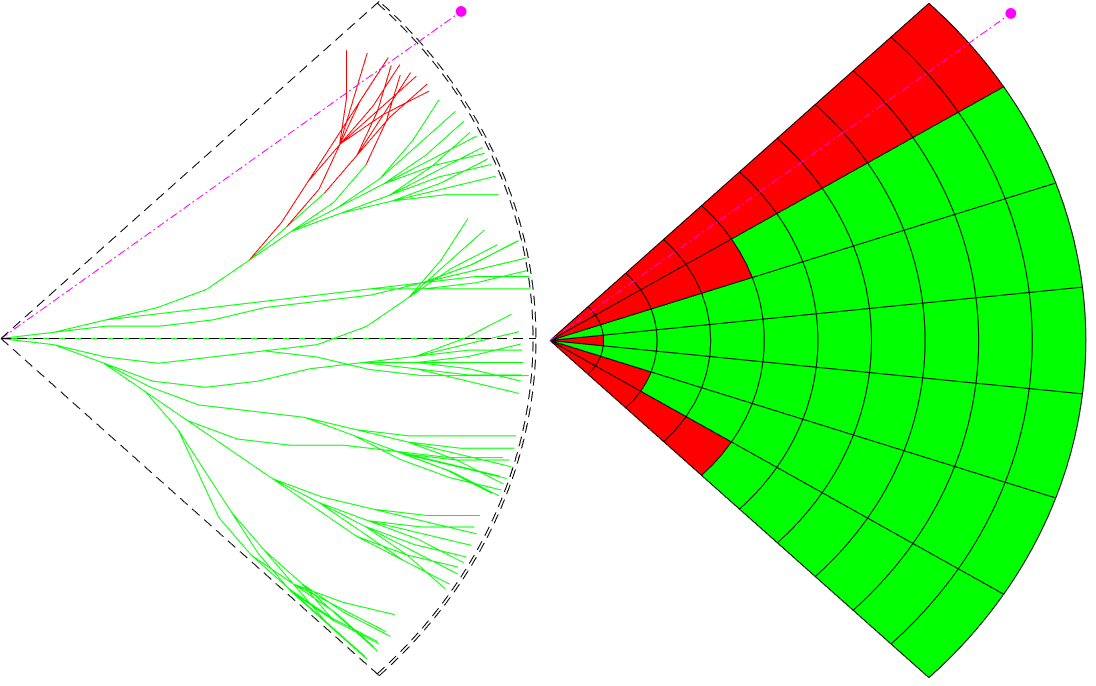
\includegraphics[width=0.9\linewidth,height=94pt,keepaspectratio]{\FIGDIR/RE016RightPlaneHeadin01} 
            \caption{$\alpha=-38.25^\circ$}
            \label{fig:ruleRightPlaneHeading01}
        \end{subfigure}
        \begin{subfigure}{0.32\textwidth}
        	\centering
            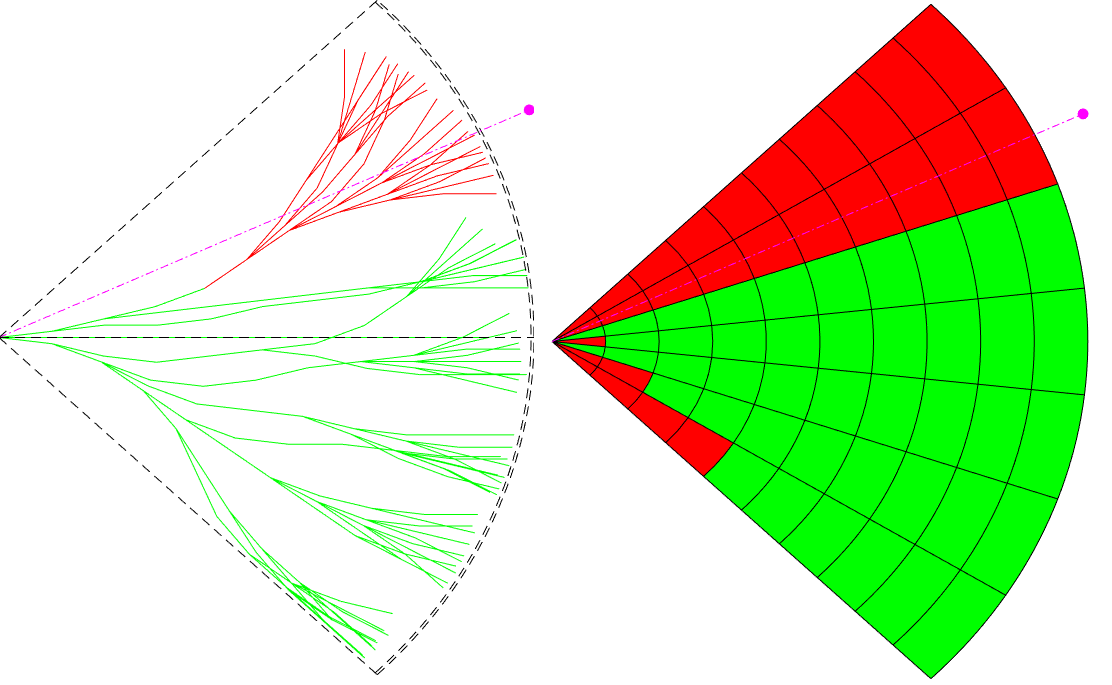
\includegraphics[width=0.9\linewidth,height=94pt,keepaspectratio]{\FIGDIR/RE17RightPlaneHeading02} 
            \caption{$\alpha=-25.5^\circ$}
            \label{fig:ruleRightPlaneHeading02}
        \end{subfigure}
        \begin{subfigure}{0.32\textwidth}
        	\centering
            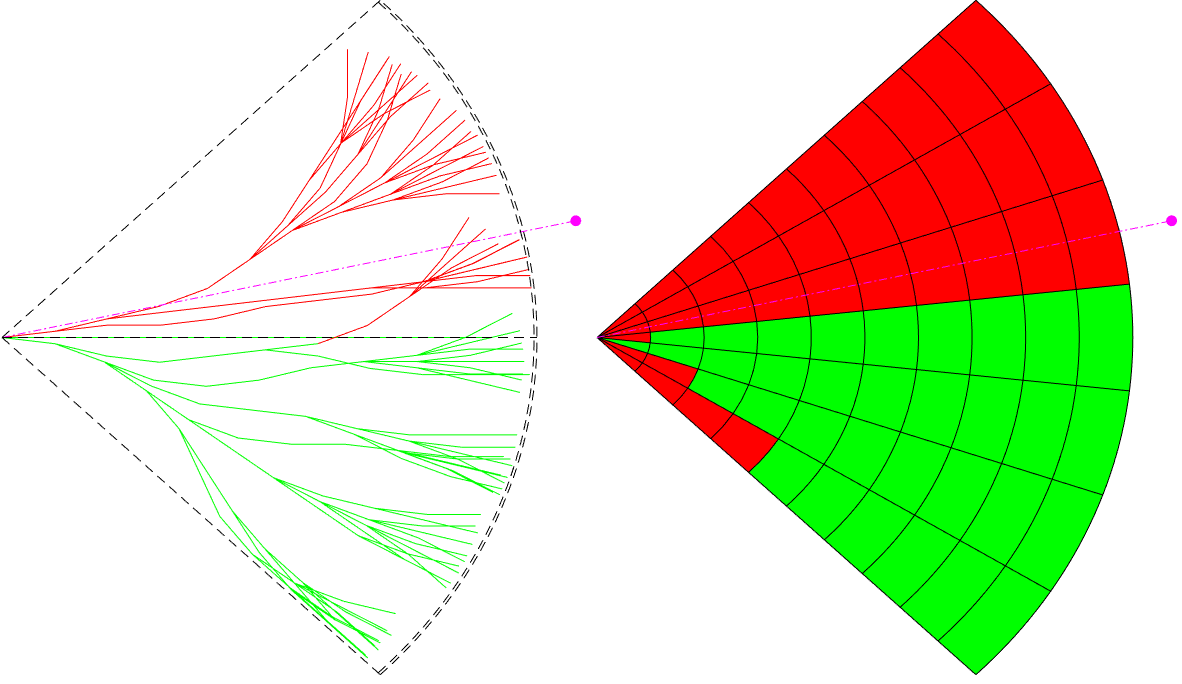
\includegraphics[width=0.9\linewidth,height=94pt,keepaspectratio]{\FIGDIR/RE018RightPlaneHeading03} 
            \caption{$\alpha=-12.75^\circ$}
            \label{fig:ruleRightPlaneHeading03}
        \end{subfigure}
        \\
        \begin{subfigure}{0.32\textwidth}
        	\centering
            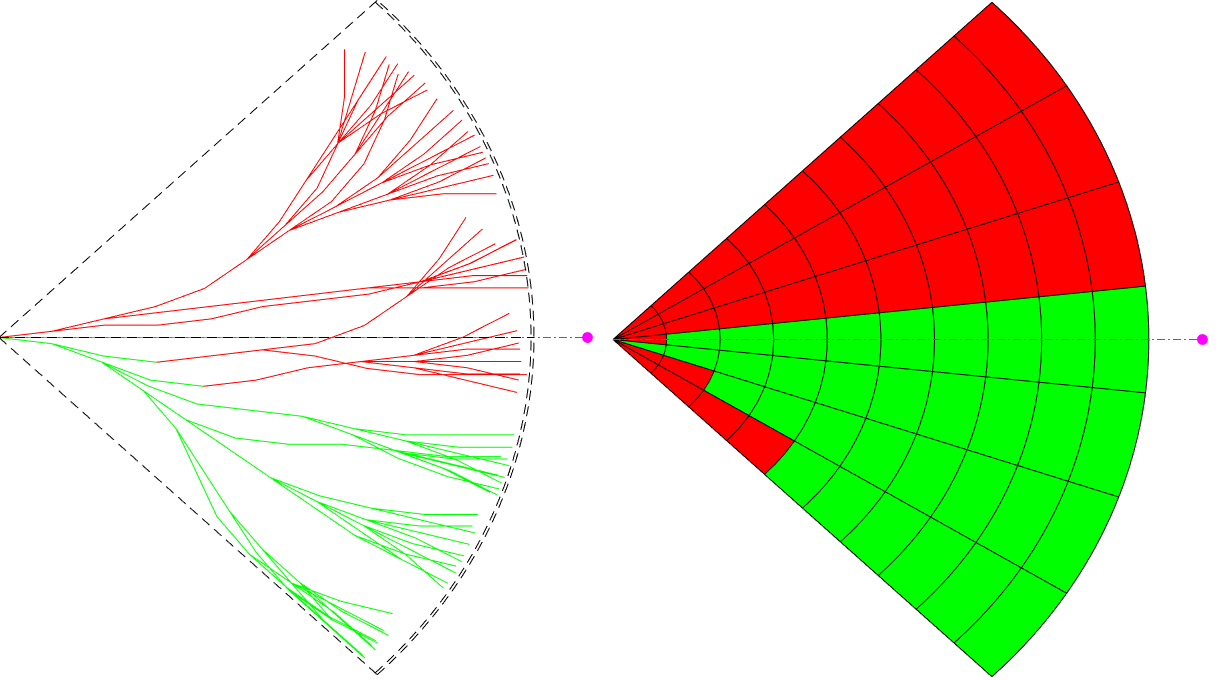
\includegraphics[width=0.9\linewidth,height=94pt,keepaspectratio]{\FIGDIR/RE019RightPlaneHeading04} 
            \caption{$\alpha=0^\circ$}
            \label{fig:ruleRightPlaneHeading04}
        \end{subfigure}
        \begin{subfigure}{0.32\textwidth}
        	\centering
            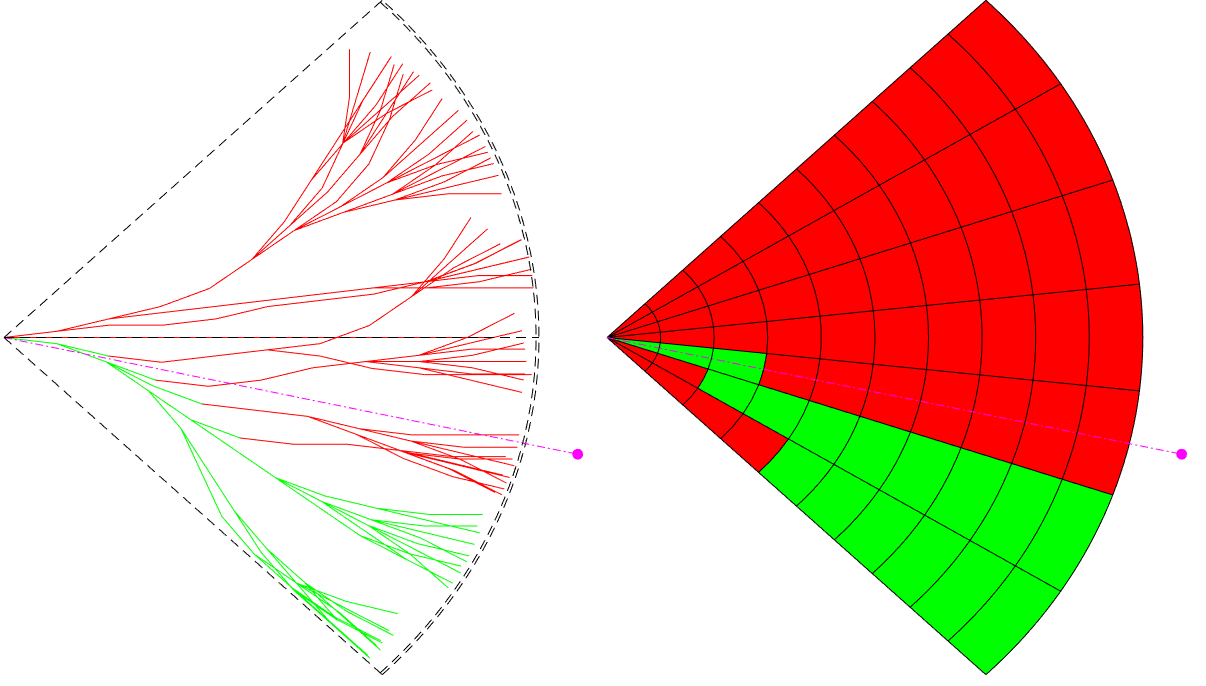
\includegraphics[width=0.9\linewidth,height=94pt,keepaspectratio]{\FIGDIR/RE020RightPlaneHeading05} 
            \caption{$\alpha=12,75^\circ$}
            \label{fig:ruleRightPlaneHeading05}
        \end{subfigure}
        \begin{subfigure}{0.32\textwidth}
        	\centering
            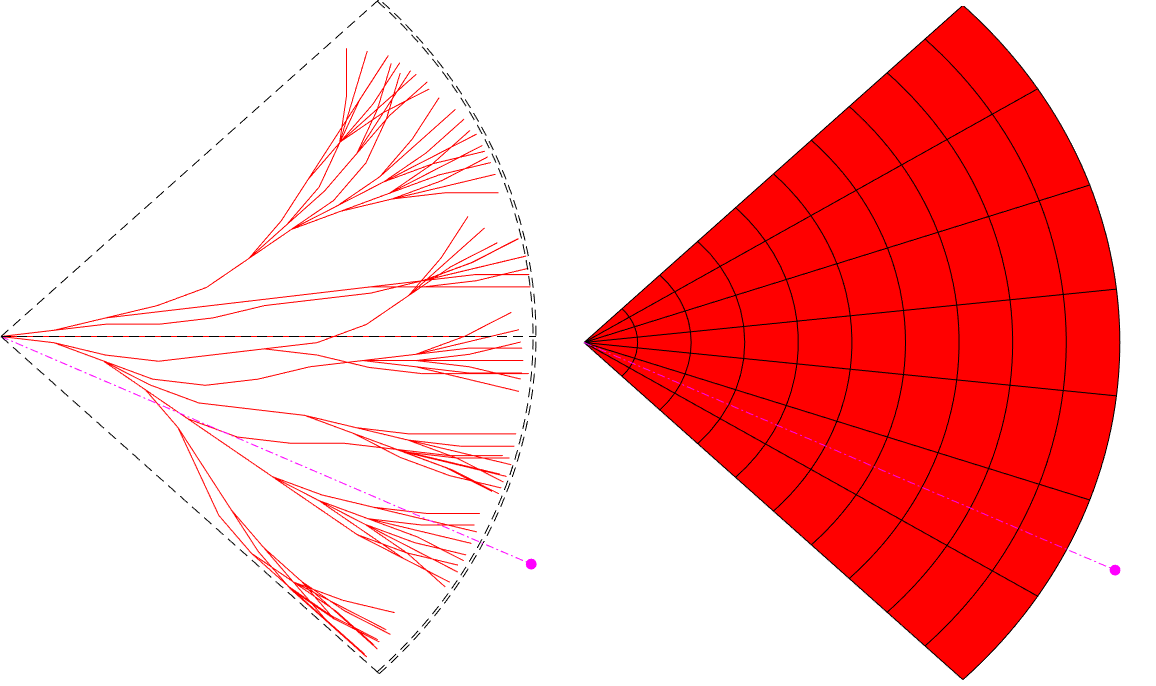
\includegraphics[width=0.9\linewidth,height=94pt,keepaspectratio]{\FIGDIR/RE021RightPlaneHeading07} 
            \caption{$\alpha=25.5^\circ$}
            \label{fig:ruleRightPlaneHeading06}
        \end{subfigure}
        \caption{Right plane heading rule evaluation for various angles of approach $\alpha$.}        
        \label{fig:ruleRightPlaneHeadingGeneral}
    \end{figure}
    
    \noindent Figure \ref{fig:ruleRightPlaneHeadingGeneral}. shows \emph{enabled} (green line) and \emph{disabled} (red lines) \emph{trajectories} (left sub-figure). These trajectories are divided according to \emph{separation line} (magenta dashed line), given by \emph{vehicle position} and \emph{collision point} (magenta circle). \emph{Space segmentation} (right subfigure) show \emph{reachable} (green fill) \emph{unreachable} (red fill) space. Situation is shown for various \emph{collision point angles of approach} $\alpha$.
    
    Rule for right plane heading check is summarized in table \ref{tab:ruleRightPlaneHeading}.   
    \begin{tabularx}{\textwidth}{|X|X|X|}
    \hline\multicolumn{3}{|X|}{
        \begin{minipage} [t] {0.95\textwidth} 
            \emph{Invocation:} Invoked by other \emph{maneuver rules}.\\\\
            \emph{Objective:} Disable all \emph{trajectories} in \emph{Navigation grid`s reach set} which are:
            \begin{enumerate}
                \item \emph{Heading into collision zone}
                \item \emph{Leading into collision zone}
            \end{enumerate}
            \rule{0pt}{0pt}
        \end{minipage}}\\
    \hline%\multicolumn{3}{X|}{Context & Condition & Application}\\
    \hline
        \emph{Context} & \emph{Condition} & \emph{Application}\\
    \hline
        \begin{minipage} [t] {0.3\textwidth}
            UAS Navigation Grid,\\
            Collision point (LOC)
            \vspace{2mm}
        \end{minipage}&
        \begin{minipage} [t] {0.3\textwidth}
            There are feasible trajectories in Navigation Grid.
            \vspace{2mm}
        \end{minipage}&
        \begin{minipage} [t] {0.3\textwidth}
            Disable trajectories in Navigation Grid.
            \vspace{2mm}
        \end{minipage}\\
    \hline
            \caption{Right plane heading rule definition.}
    \label{tab:ruleRightPlaneHeading}
    \end{tabularx}     
    
\subsection{Rule: Enforce safety margin}\label{sec:ruleEnforceSafetyMargin}
    \noindent Rule \ref{tab:ruleRightPlaneHeading}. checks right plane heading for single mass point along \emph{trajectiories}. Rule needs to account \emph{body mass} of \emph{intruder} and UAS, other factors like safe distance, regulations etc. All mentioned factors are included in \emph{safety margin}. \emph{Safety margin} is applied as \emph{radius ball} around \emph{collision point}. 
    
    \emph{Collision point} can be mapped from \emph{global coordinate frame} to \emph{reach set coordinate frame}, based on UAS \emph{position and orientation} in \emph{decision time}. Then comparison of distance between \emph{collision point} and every \emph{trajectory decision point} is trivial. 
    
    \emph{Trajectory feasibility condition}  for \emph{non-controlled airspace} (\ref{eq:ruleSafetyMarginCondition}) is given as follow:
    
    \begin{equation}\label{eq:ruleSafetyMarginCondition}
        \forall position \in trajectory, \quad distance(position,collision point) \ge safetyMargin
    \end{equation}
    
    \noindent\emph{Controlled airspace} must maintain \emph{well clear condition}. To enforce protective barrel around \emph{collision point} one must compare \emph{global coordinates}.
    \emph{Trajectory feasibility condition}  for \emph{controlled airspace} (\ref{eq:ruleSafetyMarginConditionControlled}) is given as follow:
    
    \begin{equation}\label{eq:ruleSafetyMarginConditionControlled}
        \begin{aligned}
            \forall position \in &trajectory,\\
            &XYdistance(position,collisionPoint) \ge safetyMargin\\
            &flightLevelStart \ge Z(position) \ge flightLevelEnd
        \end{aligned}
    \end{equation}
    
    \begin{figure}[H]
    	\centering
        \begin{subfigure}{0.32\textwidth}
        	\centering
            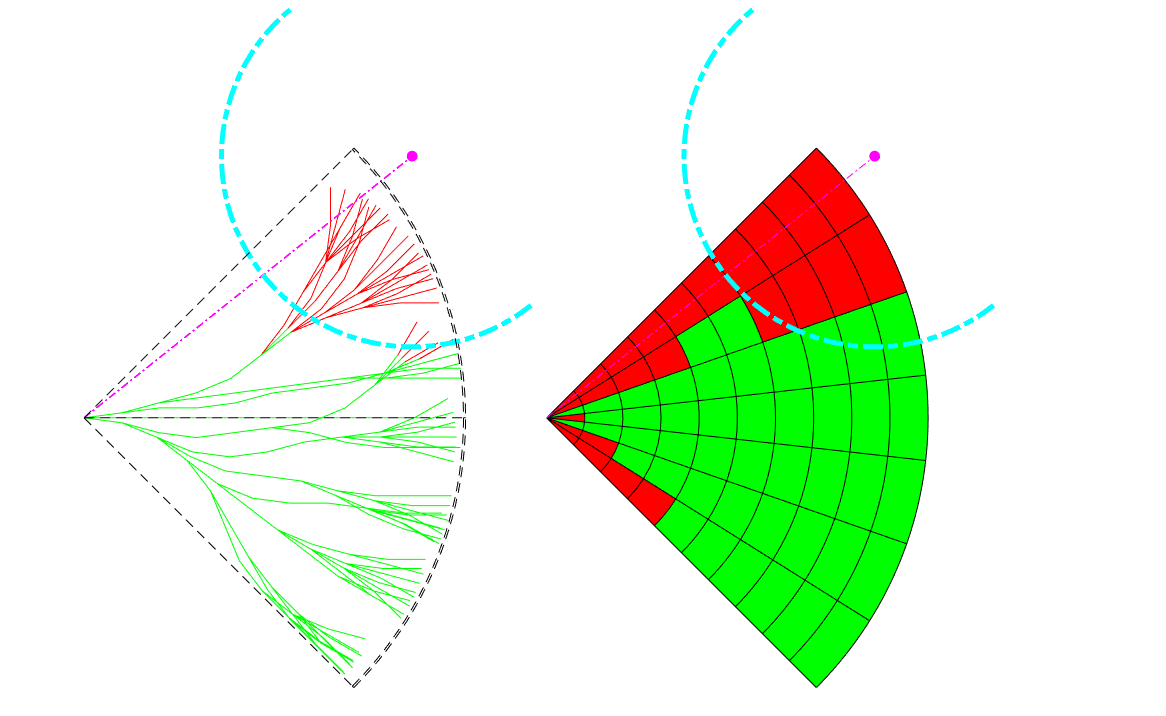
\includegraphics[width=0.9\linewidth]{\FIGDIR/RE023EnforceSafetyMargin01} 
            \vfill
            \caption{$\alpha=-38.25^\circ$}
            \label{fig:ruleEnforceSafetyMargin01}
        \end{subfigure}
        \begin{subfigure}{0.32\textwidth}
        	\centering
            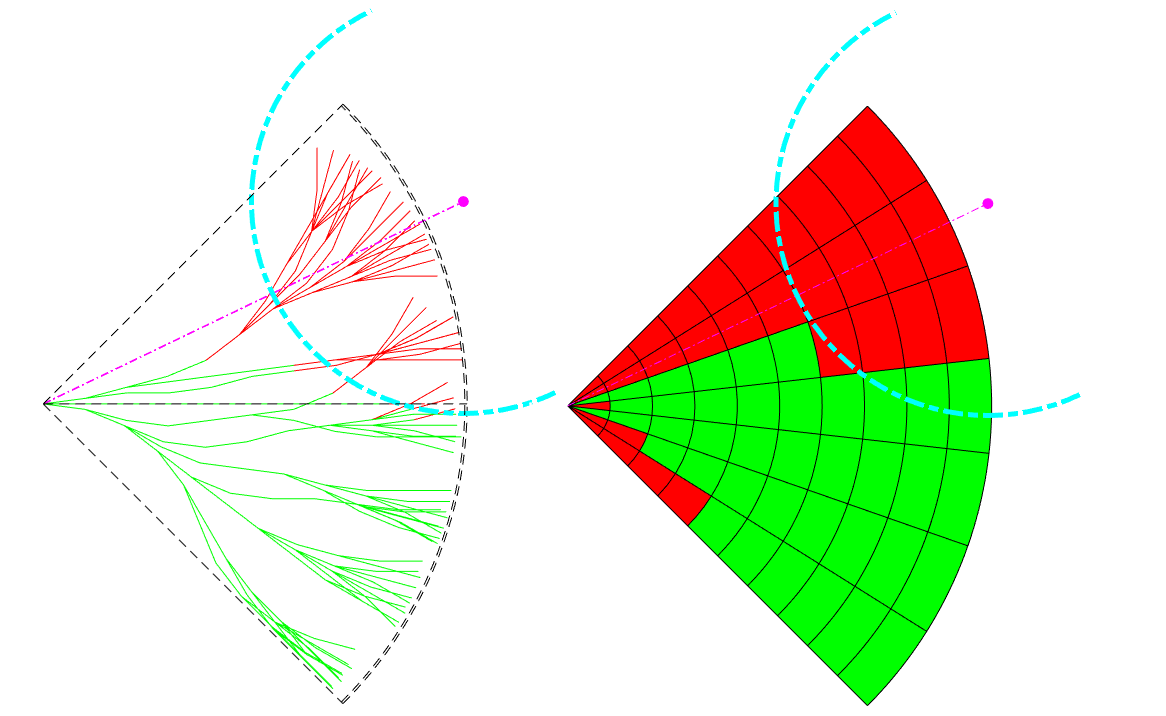
\includegraphics[width=0.9\linewidth]{\FIGDIR/RE024EnforceSafetyMargin02} 
            \vfill
            \caption{$\alpha=-25.5^\circ$}
            \label{fig:ruleEnforceSafetyMargin02}
        \end{subfigure}
        \begin{subfigure}{0.32\textwidth}
        	\centering
            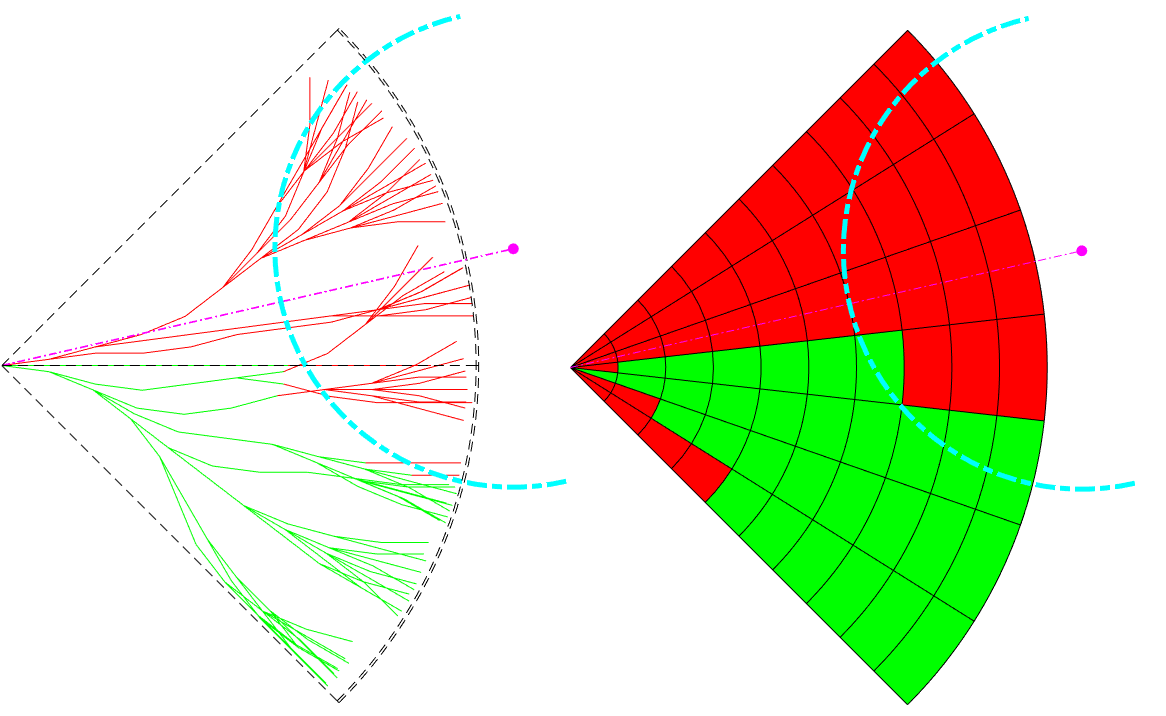
\includegraphics[width=0.9\linewidth]{\FIGDIR/RE025EnforceSafetyMargin03} 
            \vfill
            \caption{$\alpha=-12.75^\circ$}
            \label{fig:ruleEnforceSafetyMargin03}
        \end{subfigure}
        \\
        \begin{subfigure}{0.32\textwidth}
        	\centering
            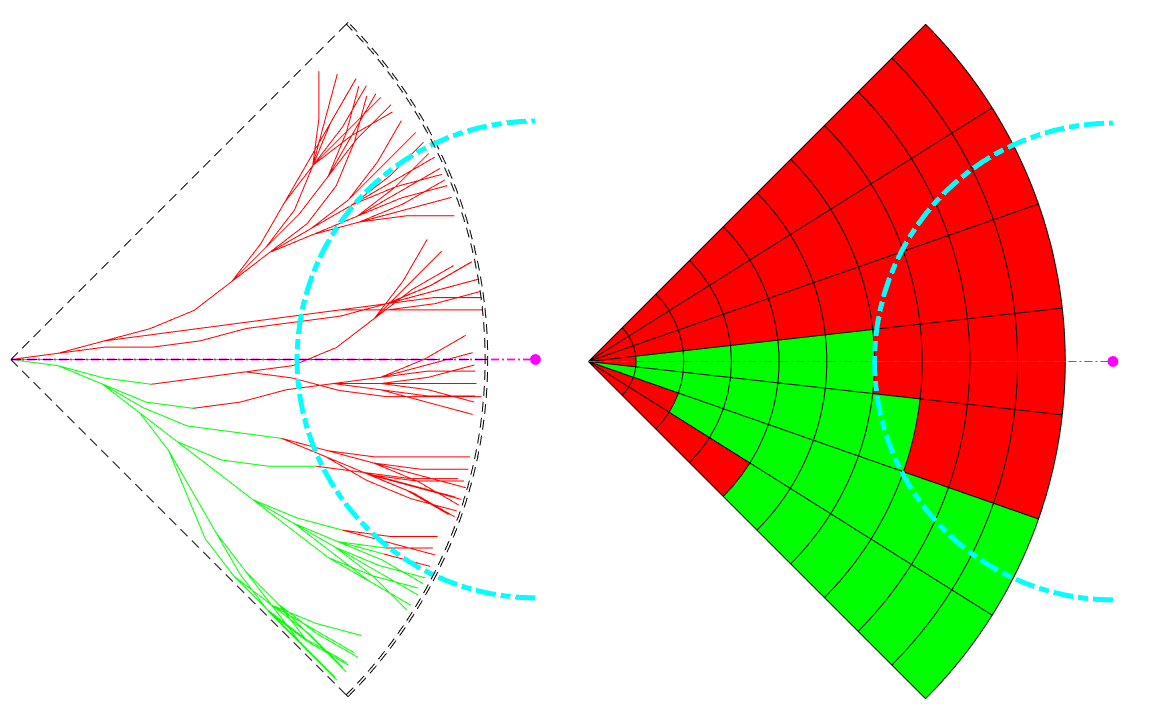
\includegraphics[width=0.9\linewidth]{\FIGDIR/RE026EnforceSafetyMargin04} 
            \vfill
            \caption{$\alpha=0^\circ$}
            \label{fig:ruleEnforceSafetyMargin04}
        \end{subfigure}
        \begin{subfigure}{0.32\textwidth}
        	\centering
            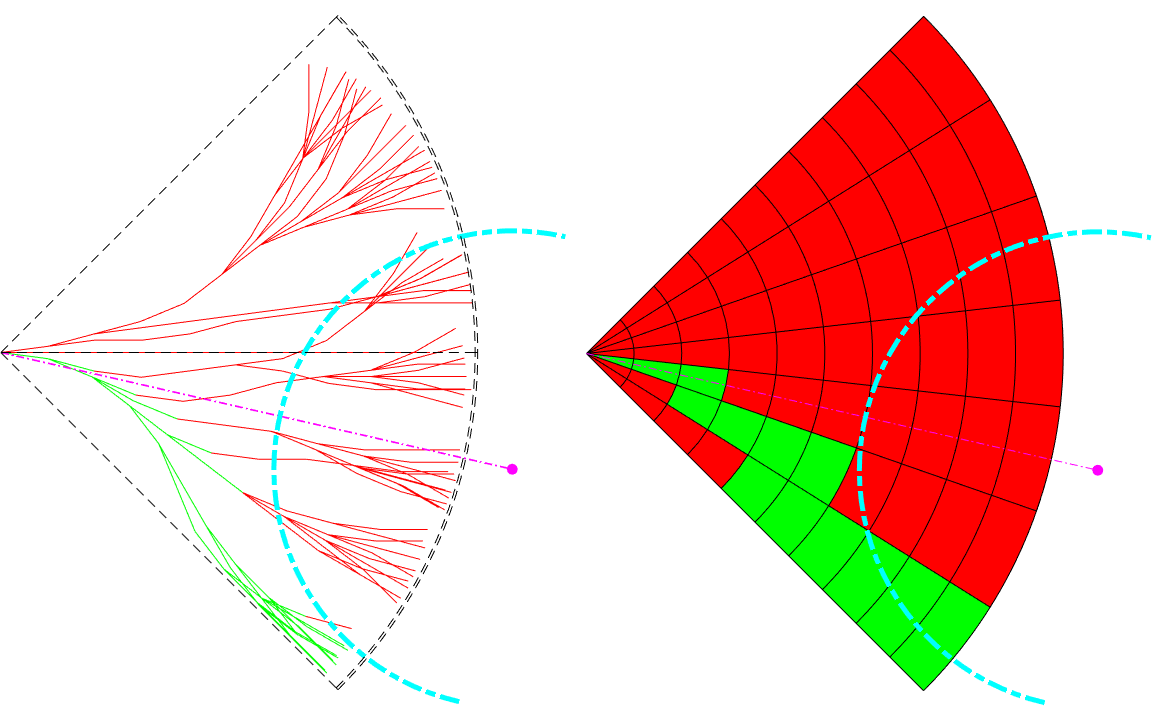
\includegraphics[width=0.9\linewidth]{\FIGDIR/RE027EnforceSafetyMargin05} 
            \vfill
            \caption{$\alpha=12,75^\circ$}
            \label{fig:ruleEnforceSafetyMargin05}
        \end{subfigure}
        \begin{subfigure}{0.32\textwidth}
        	\centering
            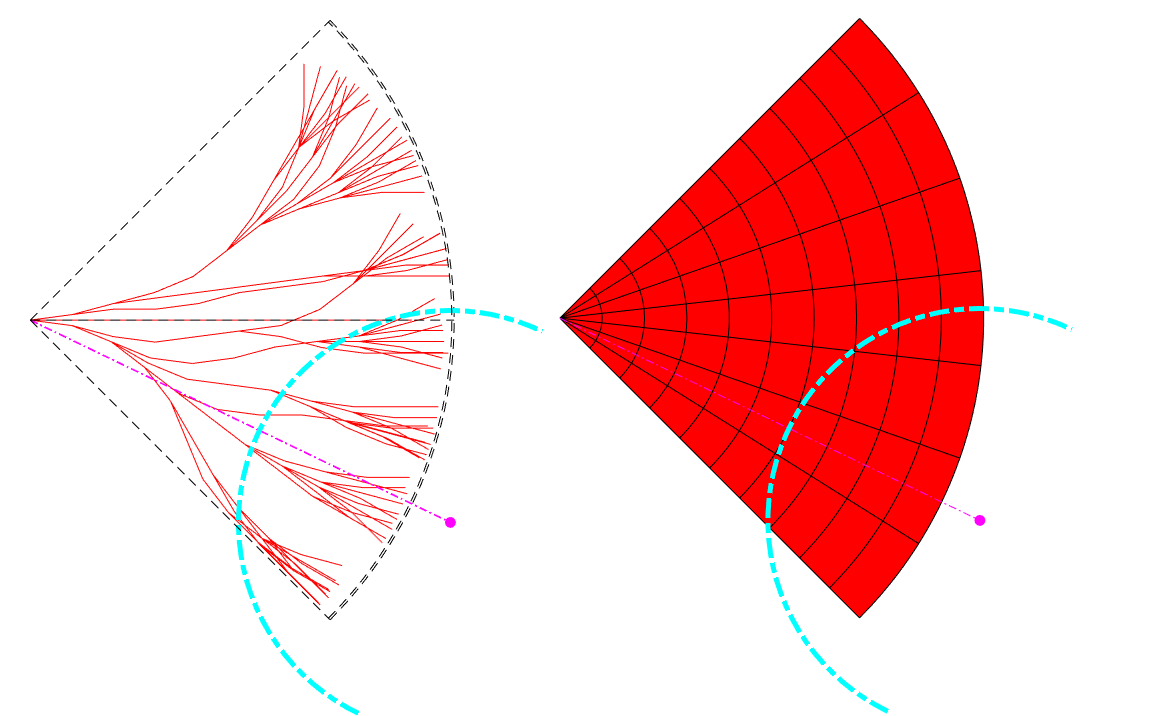
\includegraphics[width=0.9\linewidth]{\FIGDIR/RE028EnforceSafetyMargin06} 
            \vfill
            \caption{$\alpha=25.5^\circ$}
            \label{fig:ruleEnforceSafetyMargin06}
        \end{subfigure}
        \caption{Enforce safety margin rule evaluation for various angles of approach $\alpha$.}        
        \label{fig:ruleEnforceSafetyMarginGeneral}
    \end{figure}
    
    \noindent Figure \ref{fig:ruleEnforceSafetyMarginGeneral}. shows \emph{enabled} (green line) and \emph{disabled} (red lines) \emph{trajectories} (left sub-figure). These trajectories are divided according to \emph{separation line} (magenta dashed line), given by \emph{vehicle position} and \emph{collision point} (magenta circle). More trajectories are disabled due to \emph{safety  margin} (teal dashed line) around the  \emph{collision point}. \emph{Space segmentation} (right subfigure) show \emph{reachable} (green fill) \emph{unreachable} (red fill) space. Situation is shown for various \emph{collision point angles of approach} $\alpha$.
    
    Rule for safety margin check is summarized in table \ref{tab:ruleEnforceSafetyMargin}.   

    \begin{tabularx}{\textwidth}{|X|X|X|}
    \hline\multicolumn{3}{|X|}{
        \begin{minipage} [t] {0.95\textwidth} 
            \emph{Invocation:} Invoked by other \emph{maneuver rules}.\\\\
            \emph{Objective:} Based on type of airspace, for given \emph{collision point} and \emph{safety margin} disable trajectories in:
            \begin{enumerate}
                \item Ball radius for \emph{non-controlled} airspace (\ref{eq:ruleSafetyMarginCondition}).
                \item Well clear barrel \emph{controlled} airspace (\ref{eq:ruleSafetyMarginConditionControlled}).
            \end{enumerate}
            \rule{0pt}{0pt}
        \end{minipage}}\\
    \hline%\multicolumn{3}{X|}{Context & Condition & Application}\\
    \hline
        \emph{Context} & \emph{Condition} & \emph{Application}\\
    \hline
        \begin{minipage} [t] {0.3\textwidth}
            UAS Navigation Grid\\
            Collision point\\
            Safety Margin\\
            \vspace{2mm}
        \end{minipage}&
        \begin{minipage} [t] {0.3\textwidth}
            There are feasible trajectories for condition application.
            \vspace{2mm}
        \end{minipage}&
        \begin{minipage} [t] {0.3\textwidth}
            Disable trajectories in Navigation Grid.
            \vspace{2mm}
        \end{minipage}\\
    \hline
            \caption{Enforce safety margin rule definition.}
    \label{tab:ruleEnforceSafetyMargin}
    \end{tabularx}
